\documentclass[tikz, preview]{standalone}
\usepackage{amsfonts, amsthm, amssymb, amsmath, stmaryrd, etoolbox}
\usepackage{tikz}
\usetikzlibrary{matrix,arrows}
\begin{document}
%%%%%%%%%%%%%%%%%	
%%%%%%%%%%%%%%%%%
\[
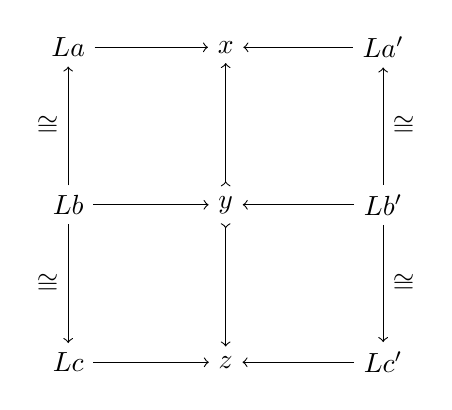
\begin{tikzpicture}
%	\draw [help lines, step=0.2, color=blue!10] (-5,-5) grid (5,5); % grid
	%
	\node (a) at (-1,1) {$ L a $};
	\node (x) at (1,1) {$ x $};
	\node (a') at (3,1) {$ L a' $};
	\node (b) at (-1,-1) {$ L b $};
	\node (y) at (1,-1) {$ y $};
	\node (b') at (3,-1) {$ L b' $};
	\node (c) at (-1,-3) {$ L c $};
	\node (z) at (1,-3) {$ z $};
	\node (c') at (3,-3) {$ L c' $};
	%
	\draw [->] (a) to (x);
	\draw [->] (a') to (x);
	\draw [->] (b) to (y);
	\draw [->] (b') to (y);
	\draw [->] (c) to (z);
	\draw [->] (c') to (z);
	\draw [->] (b) to node [left] {$ \cong $} (a);
	\draw [->] (b) to node [left] {$ \cong $} (c);
	\draw [>->] (y) to (x);
	\draw [>->] (y) to (z);
	\draw [->] (b') to node [right] {$ \cong $} (a');
	\draw [->] (b') to node [right] {$ \cong $} (c');
\end{tikzpicture}
\]
%%%%%%%%%%%%%%%%%
%%%%%%%%%%%%%%%%%
\end{document}
